% ECI v4.7 — svjour3 port for EPJ C submission
% Single-file manuscript (all \input{} resolved inline); bibliography at ../../paper/eci.bib
% Compile: latexmk -pdf eci_svjour3.tex
% Requires local: svjour3.cls, svepjc3.clo, spphys.bst (vendored beside this file).
\documentclass[epjc3,twocolumn]{svjour3}

\smartqed
\usepackage{graphicx}
\usepackage[utf8]{inputenc}
\usepackage[T1]{fontenc}
\usepackage{amsmath,amssymb}
\usepackage{physics}
\usepackage{xcolor}
\usepackage{hyperref}
\hypersetup{colorlinks=true,linkcolor=blue,citecolor=blue,urlcolor=blue}

% Convention note: Faraoni sign convention throughout (xi = 1/6 conformal).
% Reduced Planck mass M_P = 2.435 x 10^18 GeV.

\journalname{Eur. Phys. J. C}

\begin{document}

\title{ECI --- Entanglement, Complexity, Information:\\
a framework paper threading six programs into one predictive canvas}
\titlerunning{ECI framework}

\author{Kevin Remondi\`ere%
\thanks{\email{kevin.remondiere@gmail.com}.
Permanent archive: Zenodo DOI \href{https://doi.org/10.5281/zenodo.19686399}{10.5281/zenodo.19686399} (CERN Data Centre, CoreTrustSeal). Source repository: \url{https://github.com/AIdevsmartdata/crossed-cosmos}.}%
}
\authorrunning{K. Remondi\`ere}

\institute{Independent Researcher (ORCID 0009-0008-2443-7166)}

\date{Received: date / Accepted: date}

\abstract{%
We propose \textbf{ECI} (Entanglement--Complexity--Information), a phenomenological architecture assembling six independently-established research programs (2022--2026) into a unified predictive canvas: (i) type-II observer-dependent von Neumann algebras via the QRF crossed product~\cite{CLPW2023,DEHK2025a,DEHK2025b}; (ii) DESI DR2 dynamical-dark-energy preference at 2.6--3.9$\sigma$~\cite{DESIDR2} addressed by non-minimally coupled thawing quintessence $\xi_\chi R \chi^2/2$~\cite{Ye2025,Wolf2025,PanYe2026}, with the v5.0 4-chain MPI MCMC on DR2~BAO + Pantheon+ yielding $\xi_\chi=0.003^{+0.065}_{-0.070}$ (68\% CL, $\chi_0=M_P/10$, $R-1=0.036$, Savage--Dickey $\mathrm{BF}_{01}\simeq 1$; posterior prior-dominated at DR2+SN precision, see \S\ref{sec:xi_constraints}); (iii) the $H_0$ tension reduced to $\sim 2\sigma$ by Early Dark Energy with $f_{\mathrm{EDE}} = 0.09 \pm 0.03$~\cite{PoulinSmith2026}; (iv) the Dark Dimension scenario $c' \simeq 0.05$~\cite{Bedroya2025} as a microscopic DM candidate; (v) Cryptographic Censorship as a working-conjecture bulk-geometry criterion, linked through the observer-dependent reading of A1 (\S\ref{sec:thesis}) and made operational through an explicit toy dS/FLRW dictionary (\S\ref{sec:A3-dictionary})~\cite{CryptoCensorship}; (vi) persistent-homology diagnostics of primordial non-Gaussianity~\cite{Yip2024}. ECI is an architectural synthesis, not a derivation.%
\keywords{dark energy \and quintessence (non-minimal coupling) \and von Neumann algebras \and early dark energy \and persistent homology cosmology}
\PACS{98.80.-k \and 04.62.+v \and 11.25.Tq}
}

\maketitle

\section{Axioms}\label{sec:axioms}

\noindent\textbf{A1 --- Observer-dependent algebra.}
To each QRF $\mathcal{R}$ attached to a geodesic observer we associate a type-II von Neumann algebra obtained by crossed product: type II$_1$ for static de Sitter patches~\cite{CLPW2023}, type II$_\infty$ for Schwarzschild--de Sitter Killing horizons. The generalised entropy
\begin{equation}
S_{\mathrm{gen}}[\mathcal{R}] = \frac{A}{4 G_N} + S_{\mathrm{matter}}
\end{equation}
is a functor on the QRF category, well-defined modulo inner automorphism~\cite{DEHK2025a,DEHK2025b}.

\smallskip
\noindent\textbf{A2 --- Emergent geometry.}
Einstein's equations follow from $\delta Q = T_U \, \delta S_{\mathrm{gen}}$ on local Rindler horizons~\cite{Jacobson1995}, with a non-perturbative GSL~\cite{FaulknerSperanza2024,Kirklin2025}.

\smallskip
\noindent\textbf{A3 (working conjecture) --- Cryptographic Censorship.}
Any holographic CFT state whose dynamics restricted to a region $\mathcal{C}$ is $\varepsilon$-approximately a $k$-design admits a bulk dual containing an event horizon inside $\mathcal{C}$~\cite{CryptoCensorship}. The existence of pseudorandom unitaries, constructed from quantum one-way functions~\cite{MaHuang2025}, makes the criterion non-vacuous at the CFT level; the associated $k$-design saturation timescale is rigorous for random local unitaries~\cite{Haferkamp2022}. We flag A3 as a \emph{working conjecture} rather than a theorem in the cosmological setting: the original result is proven in AdS/CFT, and its transposition to de Sitter or FLRW horizons is not established. A concrete toy dictionary making the intended CFT$\to$cosmology map explicit (and its single testable consequence) is given in \S\ref{sec:A3-dictionary}; all cosmological uses of A3 below should be read as consequences of that dictionary.

\smallskip
\noindent\textbf{A4 --- Two-field scalar sector with non-minimal coupling.}
\begin{itemize}
\item $\phi$: axion-like EDE, $V_\phi = m^2 f^2 [1-\cos(\phi/f)]^3$ active at $z_c \sim 3500$~\cite{Poulin2019}.
\item $\chi$: late thawing quintessence, $V_\chi = V_0 e^{-\alpha \chi / M_P}$ with non-minimal coupling $\xi_\chi R \chi^2 / 2$~\cite{Ye2025,Wolf2025,PanYe2026}.
\end{itemize}
The joint $(\phi,\chi)$ prior is degenerate~\cite{WangPiao2025}: EDE and thawing cannot be separated by BAO+SN alone. We treat $\chi$ as a four-dimensional effective scalar; whether $\chi$ descends from a bulk mode of the extra-dimensional sector of A5 or is a decoupled zero-mode is a model-building choice whose consequences are discussed in \S3.6.

\smallskip
\noindent\textbf{A5 --- Dark Dimension.}
The species scale associated with the light KK tower obeys
\begin{equation}
\Lambda_{\mathrm{sp}}(H) = M_P \left( \frac{H}{M_P} \right)^{c'},
\label{eq:speciesH}
\end{equation}
with $c' = 1/6$ at the species scale~\cite{Montero2022,AAL2023} (used as the primary value in \S\ref{sec:xi_constraints}/\S3.6), and $c' \simeq 0.05$ as the de-Sitter-slope convention~\cite{AAL2025,OoguriVafa2007} quoted for comparison only; the species-scale exponent follows from $M_* \sim \Lambda^{1/12} M_P^{2/3}$ (Montero et al.\ Eq.~2.2) with $H^2 \sim \Lambda / M_P^2$.
A mesoscopic extra dimension, $\ell \in [0.1, 10] \, \mu\mathrm{m}$, follows. The KK graviton tower (mass $\sim$ meV) is the DM candidate, subject to the fifth-force bound $c' < 0.2$ and $N_{\mathrm{eff}} = 2.86 \pm 0.13$ (ACT DR6~\cite{Calabrese2025}).

\smallskip
\noindent\textbf{A6 --- Persistent-homology complexity.}
Local complexity of the cosmological state is quantified by $\mathrm{PH}_k$ on density super-level sets~\cite{Yip2024,Calles2025}, a finer $f_{\mathrm{NL}}$ estimator than Betti numbers. At leading order in $f_{\mathrm{NL}}$, the primordial-NG shift of the Euler characteristic $\chi_{\mathrm{E}}(\nu)$ (genus statistic) at threshold $\nu$ takes the Matsubara form (observer ensemble average; see \S\ref{sec:thesis}(ii))
\begin{equation}
\langle \chi_{\mathrm{E}}(\nu) \rangle_{f_{\mathrm{NL}}} - \langle \chi_{\mathrm{E}}(\nu) \rangle_{0} \simeq \frac{f_{\mathrm{NL}}\, \sigma_0\, S_3^{\mathrm{prim}}}{6}\, H_3(\nu)\, \phi(\nu),
\label{eq:A6-euler}
\end{equation}
with $H_3$ the third probabilists' Hermite polynomial, $\sigma_0$ the field RMS, $S_3^{\mathrm{prim}}$ the primordial skewness, and $\phi$ the Gaussian density (three-dimensional, super-level-set convention)~\cite{Matsubara2003}; the persistent-homology diagnostic of~\cite{Yip2024,Calles2025} refines this Minkowski-functional signal.

% ===== section_1_5_thesis_B inlined =====
\section{A unifying reading: observer-dependent cosmology in the late-time limit}
\label{sec:thesis}

The six axioms of \S\ref{sec:axioms} admit a common reading, valid in the late-time
quasi-de~Sitter regime ($\Omega_\Lambda \gtrsim 0.7$) where every
quantitative prediction of \S\ref{sec:pheno} is formulated. The reading is \emph{not} a
derivation of the axioms and does not extend to the pre-recombination
sector (A4's EDE axion $\phi$ at $z_c\sim 3500$; BBN-level constraints on
$\xi_\chi$); those inputs remain background-level inheritances from the
external literature as in v4.6.

\subsection*{(i) The crossed-product backbone}

The type-III$_1$ algebra of quantum fields restricted to a gravitational
subregion carries no trace and no density matrices; the Chandrasekaran--
Longo--Penington--Witten (CLPW) construction~\cite{CLPW2023} and its
quantum-reference-frame (QRF) completion by De~Vuyst--Eccles--H\"ohn--
Kirklin (DEHK)~\cite{DEHK2025a,DEHK2025b} repair this by crossing with the
modular automorphism of an observer clock, yielding a type-II$_1$ algebra on
the static de~Sitter patch (II$_\infty$ on Schwarzschild--de~Sitter
Killing horizons) with a well-defined trace and an entropy reproducing
$S_{\rm gen} = A/(4G_N) + S_{\rm matter}$ up to a state-independent
constant. DEHK make the observer-dependence structural: distinct QRFs
yield distinct crossed-product algebras, distinct modular flows, and
distinct numerical values of $S_{\rm gen}$ on the same underlying bulk
state. The non-perturbative generalised second law of
Faulkner--Speranza~\cite{FaulknerSperanza2024} and
Kirklin~\cite{Kirklin2025} is formulated on exactly this type-II entropy.
The observer-dependent crossed-product construction extends to FLRW
cosmologies that are asymptotically de~Sitter~\cite{KFLS2024}, and a
microscopic dS model reproducing the observer-dependent entropy has been
proposed in~\cite{TiettoVerlinde2025}. The \emph{organising reading}
proposed here is that the effective couplings entering the late-time
phenomenology of \S\ref{sec:pheno} are observer-frame labelled, not
background quantities defined once and for all.

\subsection*{(ii) A4--A6 as observer-frame quantities}

\emph{A4 --- NMC coupling $\xi_\chi$.} The graviton kinetic matrix of the
Jordan-frame action of \S\ref{sec:action} is frame-dependent via the type-II trace
normalisation; a geodesic observer whose crossed product is built from a
different clock Hamiltonian measures $\xi_\chi^{(\mathcal R)}$. The
Cassini bound $|\xi_\chi|(\chi_0/M_P)\le 2.4\times 10^{-3}$ of
\S\ref{sec:xi_constraints} constrains the \emph{solar-system-frame} value,
which is the only value the experiment is sensitive to.

\emph{A5 --- species-scale exponent $c'$.} The tower visible to a causal
diamond is frame-labelled; $c' = 1/6$ is the asymptotic quasi-dS value
(Montero--Vafa--Valenzuela~\cite{Montero2022}; AAL~\cite{AAL2023})
recovered when the diamond saturates the static patch.

\emph{A6 --- persistent homology $\mathrm{PH}_k$.} The Euler-characteristic
shift of~\eqref{eq:A6-euler} is computed on a density field restricted to
an observer-accessible region. The Matsubara baseline is the ensemble
average over observer frames; the diagnostic power of $\mathrm{PH}_k$
relative to the bispectrum is accordingly a frame-averaged statement,
consistent with PRINCIPLES~\S12 (no claim beyond derivation).

\subsection*{(iii) A3 as a self-consistency condition}

Cryptographic Censorship~\cite{CryptoCensorship}, in its AdS/CFT proof,
states that boundary-restricted $\varepsilon$-approximate $k$-design
dynamics implies a bulk event horizon. Under the present reading, A3 is
not an independent axiom but the self-consistency condition bounding the
subregion on which the QRF crossed product of A1 remains well-defined:
an observer whose modular algebra sees an effectively pseudorandom state
has lost predictive access to the complement region, and an event horizon
must cap the subregion on which A4--A6 are defined. The cosmological
transposition of A3 remains a working conjecture quarantined in
Appendix~A (PRINCIPLES~\S8); the reading does not upgrade its status.

\subsection*{(iv) Caveats and scope}

Two scope restrictions are part of the claim, not loopholes around it.

\emph{(S1) Static-patch asymptote.} CLPW is proven on the static dS
patch; DEHK extend to multi-observer QRFs on the same Killing-horizon
background. The late-time FLRW diamond approaches this asymptote with
$O(1-\Omega_\Lambda)$ corrections; the adiabatic tolerance of modular
flow to the DESI~DR2 pivot $|\dot H|/H^2 \sim O(1)$ is a \emph{heuristic}
extension, at the same footing as the Faulkner--Speranza
non-perturbative GSL.

\emph{(S2) Matter-era exclusion.} Pre-recombination A4/A5 statements
(the EDE axion $\phi$ at $z_c\sim 3500$, the BBN $\xi_\chi$ bound of
Wolf~2025~\cite{Wolf2025}) are background-level inheritances; the
observer-frame reading is not claimed for them. Their treatment under
the present reading would require a QRF extension to time-dependent FLRW
backgrounds which is an open problem in the algebraic-gravity
literature.

A joint falsifier is available: any experimental anomaly breaking the
consistency between the solar-system-frame $\xi_\chi$ (Cassini,
\S\ref{sec:xi_constraints}) and the late-time cosmological-frame
$\xi_\chi$ (DR3/LSST~Y10, Prediction~1b) beyond the static-patch
$O(1-\Omega_\Lambda)$ budget would damage the present reading without
touching the Lagrangian of \S\ref{sec:action}. The experimental precision is at least a
decade out, but the handle is not zero.

\subsection*{Status}

This section is an \emph{organising reading} of the six axioms in the
late-time quasi-dS regime, not a derivation, and does not enter the
predictive core \S\ref{sec:pheno}--\S\ref{subsec:perturb} or \S\ref{sec:pred}. The framework-genre declaration of
\S\ref{sec:axioms} is unchanged.

% ===== end section_1_5_thesis_B =====

\section{Action and field equations}\label{sec:action}

\subsection*{Conventions}
We use the mostly-plus metric signature $(-,+,+,+)$. The non-minimal-coupling sign follows the Faraoni convention~\cite{Faraoni2004}: $\xi > 0$ gives the attractive correction, appearing as $-\tfrac{1}{2}\xi R \chi^2$ in the Lagrangian and as $+\xi R\,\chi$ in the scalar field equation. The reduced Planck mass is $M_P = (8\pi G)^{-1/2} = 2.435 \times 10^{18}$ GeV. Natural units $\hbar = c = 1$ are used throughout. Time arguments are cosmic time $t$ unless otherwise stated; conformal time $\eta$ appears only in perturbation equations.

In the Faraoni sign convention (reduced Planck mass $M_P$, $\xi = 1/6$ conformal), the effective action is
\begin{align}
\mathcal{S} = \int d^4 x \sqrt{-g}\, \Big[ & \frac{M_P^2}{2} R - \tfrac{1}{2}(\partial \phi)^2 - V_\phi(\phi) \nonumber \\
& - \tfrac{1}{2}(\partial \chi)^2 - V_\chi(\chi) - \tfrac{1}{2}\xi_\chi R \chi^2 \nonumber \\
& + \mathcal{L}_{\mathrm{SM}} + \mathcal{L}_{\mathrm{KK}}[\ell; \chi] \Big] + \mathcal{S}_{\mathrm{QRF}}.
\end{align}

\textbf{Scalar equations:}
\begin{align}
\Box \phi - V_\phi'(\phi) &= 0,\\
\Box \chi - V_\chi'(\chi) - \xi_\chi R\, \chi &= 0.
\end{align}

\textbf{Einstein equations:}
\begin{equation}
G_{\mu\nu} = \frac{1}{M_P^2} \left[ T_{\mu\nu}^{\mathrm{SM}} + T_{\mu\nu}^{(\phi)} + T_{\mu\nu}^{(\chi)} + T_{\mu\nu}^{\mathrm{KK}} \right].
\end{equation}

\textbf{NMC stress tensor} (after transferring $-\xi_\chi G_{\mu\nu} \chi^2$ to the r.h.s., Faraoni Eqs. 2.12--2.13):
\begin{align}
T_{\mu\nu}^{(\chi)} = \nabla_\mu \chi \nabla_\nu \chi & - \tfrac{1}{2} g_{\mu\nu}\left[(\nabla \chi)^2 + 2 V_\chi\right] \nonumber \\
+ \xi_\chi \Big[ g_{\mu\nu} \Box(\chi^2) & - \nabla_\mu \nabla_\nu(\chi^2) - G_{\mu\nu} \chi^2 \Big].
\end{align}

\textbf{No-ghost condition:} diagonalising the kinetic matrix of the graviton--$\chi$ sector of the NMC action gives an effective Planck mass squared $M_{P,\mathrm{eff}}^2 = M_P^2 - \xi_\chi \chi^2$; positivity of the graviton kinetic term (equivalently, positivity of the scalar-sector determinant $\det K = M_{P,\mathrm{eff}}^2/2 - \xi_\chi^2 \chi^2$ at leading order) yields
$\xi_\chi \chi^2 / M_P^2 < 1$ in reduced-Planck convention~\cite{Faraoni2004}.

\section{Phenomenology}\label{sec:pheno}

\subsection{DESI DR2 --- dark energy}
The $\chi$ field with $\xi_\chi \neq 0$ crosses $w = -1$ without a ghost pathology (non-minimal kinetic term~\cite{BarceloVisser2000}). DESI DR2 central values $w_0 \approx -0.75$, $w_a \approx -0.86$~\cite{DESIDR2}. The Scherrer--Sen relation~\cite{ScherrerSen2008} $w_a / (1+w_0) \in [-1.5, 0]$ holds at minimal coupling only; for $\xi_\chi \neq 0$ the slope is modified and must be computed numerically~\cite{Sanchez2025}. A first-order analytic estimate of $w_a(w_0; \xi_\chi)$ in the NMC thawing regime is deferred to the companion computation in \texttt{derivations/w0-wa-nmc}; without it, prediction (1) in Section~\ref{sec:pred} does not distinguish ECI from wCDM inside the quoted band.

\subsection{Hubble tension}
$f_{\mathrm{EDE}} = 0.09 \pm 0.03$, $H_0 = 71.0 \pm 1.1$ km/s/Mpc under ACT DR6 + DESI DR2 + Planck + Pantheon+~\cite{PoulinSmith2026,Calabrese2025}. Residual SH0ES tension: $\sim 2\sigma$.

\subsection{Cosmological constant}
$V_\chi = V_0 e^{-\alpha \chi / M_P}$ admits a de Sitter attractor for $\alpha \lesssim \sqrt{2}$. The bound $\alpha \le \sqrt{2}$ is the standard late-time accelerating-attractor condition for an exponential scalar~\cite{Halliwell1987,CopelandLiddleWands1998}.
Reduced Planck $M_P = 2.435 \times 10^{18}$ GeV gives $\rho_\Lambda / M_P^4 \simeq 8 \times 10^{-121}$ for $\chi_0 / M_P \sim 120/\alpha$. Consistent with the Ooguri--Vafa Swampland Distance Conjecture~\cite{OoguriVafa2007}.

\subsection{Dark matter}
Dark Dimension KK tower, $m \sim$ meV, $c' \simeq 0.05$ under fifth-force bound $c' < 0.2$ and $N_{\mathrm{eff}} = 2.86 \pm 0.13$ (ACT DR6~\cite{Calabrese2025}). ISL tests at $\ell \in [0.1, 10] \, \mu$m. $\dot G / G = (-5.0 \pm 9.6) \times 10^{-15}$ yr$^{-1}$ (LLR, Biskupek--M\"uller--Torre~\cite{Biskupek2021}). We note that two BSM anomalies sometimes invoked as motivational slots for KK-tower architectures have recently dissolved: the combined Fermilab E989 final $a_\mu$ result and the 2025 Theory-Initiative lattice-QCD HVP update leave a $\sim 0.6\sigma$ residual, consistent with the Standard Model~\cite{MuonG2Final2025}; and the CMS 2024 W-mass measurement $m_W = 80360.2 \pm 9.9$ MeV reasserts SM consistency against the 2022 CDF-II outlier~\cite{CMSWmass2024}. The DM motivation for A5 therefore rests solely on the fifth-force bound and $N_{\mathrm{eff}}$, not on these now-closed BSM channels.

% ===== section_3_5_constraints inlined =====
\subsection{Solar-system and background constraints on $\xi_\chi$}\label{sec:xi_constraints}

We close two gaps identified in the dark-energy phenomenology subsection (\S\,DESI DR2): the Cassini
post-Newtonian bound on the non-minimal coupling $\xi_\chi$, and the analytic NMC generalisation
of the Scherrer--Sen thawing relation needed to assess whether Prediction~1
(Sec.~\ref{sec:pred}) actually discriminates ECI from \(w\)CDM at DESI~DR2 precision.
The full symbolic derivation is in \texttt{derivations/D7-ppn-xi-bound.py}; we quote only the
end results here.

\paragraph{PPN $\gamma-1$ from the $\xi_\chi R\chi^2/2$ coupling.}
The action  $S=\int d^4x\sqrt{-g}\left[\tfrac{M_P^2}{2}R-\tfrac12(\partial\chi)^2-V(\chi)
-\tfrac{\xi_\chi}{2} R\chi^2\right]$ is a scalar--tensor theory with
$F(\chi)=M_P^2-\xi_\chi\chi^2$ multiplying $R/2$ and canonical kinetic term $Z=1$.
Applying the weak-field, quasi-static result of Damour \& Esposito-Far\`ese
(\emph{Phys.\ Rev.\ D} 48, 3436 (1993); see also Chiba, \emph{Phys.\ Lett.\ B} 575, 1 (2003);
Hwang \& Noh, \emph{Phys.\ Rev.\ D} 71, 063536 (2005)) gives, at the local scalar background
$\chi_0$,
\begin{equation}
  \gamma-1 \;=\; -\,\frac{F'(\chi_0)^2}{Z\,F(\chi_0)+\tfrac{3}{2}F'(\chi_0)^2}
           \;=\; -\,\frac{4\,\xi_\chi^{2}\,\chi_0^{2}}
                          {\,M_P^{2}+\xi_\chi\chi_0^{2}(6\xi_\chi-1)\,}.
  \label{eq:gamma_PPN_full}
\end{equation}
(Convention: DEF 1992 / Chiba 1999 normalization for the denominator
$Z F + \tfrac{3}{2}F'^{2}$; equivalent to Will 2014 \S3.3 under
the rescaling $Z\to Z/2$, absorbed identically in the $|\xi_\chi|\ll 1$ limit.)
Expanding for $|\xi_\chi|\ll 1$ and $\chi_0\lesssim M_P$,
\begin{equation}
  \boxed{\;\gamma-1 \;\simeq\; -\,\frac{4\,\xi_\chi^{2}\,\chi_0^{2}}{M_P^{2}}
                              \;+\;\mathcal{O}(\xi_\chi^{3}).\;}
  \label{eq:gamma_PPN_lead}
\end{equation}
The limit $\xi_\chi\to 0$ returns $\gamma=1$ (General Relativity), as verified symbolically.

The result~(\ref{eq:gamma_PPN_lead}) is not new: Chiba (PRL 82, 1836, 1999; arXiv:gr-qc/9903094)
already quoted $|\xi_\chi|\lesssim 10^{-2}$ from solar-system tests for the same $\xi R\chi^{2}$
quintessence coupling, and Wolf, Garc\'{\i}a-Garc\'{\i}a, Anton \& Ferreira~\cite{Wolf2025}
recently recast this as $\xi_\chi(\chi_0/M_P)^{2}\lesssim 6\times 10^{-6}$ in a full DESI~DR2
Bayesian analysis (their Eq.~(2) in the form $F(\chi)\simeq 1-\xi\chi^{2}/M_P^{2}$).
We re-derive it here only to fix the coefficient~$4$ and the sign convention used in
Eq.~(\ref{eq:wa_NMC}) below.
Combining (\ref{eq:gamma_PPN_lead}) with the Cassini constraint~\cite{BertottiIessTortora2003}
$|\gamma-1|\lesssim 2.3\times 10^{-5}$ ($1\sigma$ envelope) yields, in the
solar-system observer frame (see \S\ref{sec:thesis}(ii)),
\begin{equation}
  |\xi_\chi|\,\frac{\chi_0}{M_P}\;\lesssim\;
  \tfrac12\sqrt{|\gamma-1|_{\max}}
  \;\approx\; 2.4\times 10^{-3}.
  \label{eq:xi_bound}
\end{equation}
For a slow-rolling thawing background with $\chi_0\!\sim\! M_P/10$ (characteristic thawing
excursion in the last $e$-fold),
\begin{equation}
  |\xi_\chi|\;\lesssim\;\xi_{\max}\;\approx\;2.4\times 10^{-2}.
  \label{eq:xi_max_numeric}
\end{equation}
The bound tightens to $|\xi_\chi|\lesssim 2\times 10^{-3}$ if $\chi_0\sim M_P$; it weakens
linearly for smaller $\chi_0$. Values $\xi_\chi\gtrsim 10^{-1}$ are thus only admissible if the
quintessence field is strongly subdominant at $z=0$, or if a screening mechanism suppresses the
local coupling.

\paragraph{NMC extension of Scherrer--Sen.}
At minimal coupling, thawing quintessence lies on the one-parameter track
$w_a=-A(\Omega_\Lambda)(1+w_0)$ with $A\!\to\! 24/7$ in matter domination and
$A(0.7)\simeq 1.58$ today~\cite{ScherrerSen2008}. Inserting the NMC modification to the
Klein--Gordon equation, $3H\dot\chi=-V'-\xi_\chi R\chi$, and expanding to first order in
$\xi_\chi$ around the slow-roll exponential $V(\chi)=V_0e^{-\alpha\chi/M_P}$ with
$\alpha=\sqrt{3(1+w_0)}$ yields (\texttt{derivations/D4-wa-w0-nmc.py} for the matter-era
coefficient, \texttt{D7-ppn-xi-bound.py} for the $\Omega_\Lambda$-dependence)
\begin{equation}
  \boxed{\;w_a\;=\;-A(\Omega_\Lambda)\,(1+w_0)
                 \;+\;B(\Omega_\Lambda)\,\xi_\chi\,\sqrt{1+w_0}\,
                      \frac{\chi_0}{M_P}\;+\;\mathcal{O}(\xi_\chi^{2}),\;}
  \label{eq:wa_NMC}
\end{equation}
where $B(\Omega_\Lambda)$ is the numerical coefficient tabulated in
Table~\ref{tab:B_of_OmegaL} below, obtained by full NMC-Friedmann + Klein--Gordon
integration in \texttt{derivations/D13-wa-numerical-full.py}. The limit
$\xi_\chi\to 0$ reproduces $w_a=-A(\Omega_\Lambda)(1+w_0)$ (Scherrer--Sen
2008). The first-order $\xi_\chi$ correction, with the full numerical
coefficient $B_{\mathrm{num}}(\Omega_\Lambda)$, has --- to our knowledge ---
not appeared in the NMC-thawing literature surveyed
(Ye~et~al.~\cite{Ye2025}; Pan~\&~Ye~\cite{PanYe2026}; Wolf~et~al.~\cite{Wolf2025}),
which uses either EFTofDE or purely numerical Bayesian fits.

\begin{table}[h]
\centering
\caption{Numerical NMC coefficient $B_{\mathrm{num}}(\Omega_\Lambda)$ from the
self-consistent NMC-Friedmann + Klein--Gordon background integration
(\texttt{derivations/D13-wa-numerical-full.py}), compared with the D7/D9
heuristic $B_{\mathrm{heur}}(\Omega_\Lambda)\equiv(8/\sqrt3)A(\Omega_\Lambda)$.
Statistical uncertainty is the 1$\sigma$ error on the linear fit
$\Delta w_a = B\,\xi_\chi\sqrt{1+w_0}\,(\chi_0/M_P)$ over the
$\xi_\chi\in\{{-}0.024,{-}0.01,0,{+}0.01,{+}0.024\}\times\chi_0\in\{M_P/20,M_P/10,M_P/5\}$ grid.}
\label{tab:B_of_OmegaL}
\begin{tabular}{cccc}
\hline
$\Omega_\Lambda$ & $A(\Omega_\Lambda)$ & $B_{\mathrm{heur}}$ & $B_{\mathrm{num}}$ \\
\hline
0.5 & 2.35 & 10.85 & $9.00\pm1.05$ \\
0.6 & 1.94 &  8.96 & $9.18\pm1.16$ \\
0.7 & 1.58 &  7.30 & $9.05\pm1.18$ \\
0.8 & 1.23 &  5.68 & $8.11\pm1.16$ \\
\hline
\end{tabular}
\end{table}

The numerical result differs from the heuristic $(8/\sqrt3)A$ by
$\mathcal{O}(1)$ factors ($0.83\to 1.43$ across the range): $B_{\mathrm{num}}$
is nearly \emph{flat} in $\Omega_\Lambda$ (around $\sim 9$) rather than
tracking $A(\Omega_\Lambda)$. The heuristic is accurate to 5\% only near
$\Omega_\Lambda\simeq 0.6$ and underestimates $B$ by $\sim\!25\%$ at
$\Omega_\Lambda=0.7$ (DR2--DR3 era) and $\sim\!43\%$ at
$\Omega_\Lambda=0.8$ (late-DR3 / LSST era). The sign and the
$\sqrt{1+w_0}\,(\chi_0/M_P)$ scaling are confirmed; the discrepancy
originates from the finite-$\Omega_\Lambda$ propagation of the matter-era
ratio (Caveat~2 below), which is now closed numerically.

\paragraph{Combined constraint on the $(w_0,w_a)$ plane.}
Figure~\ref{fig:D7} overlays three ingredients: (i) the DESI~DR2 + CMB + DESY5~\cite{DESY5} $1\sigma$ and
$2\sigma$ contours centred on $(w_0,w_a)=(-0.752,-0.86)$ with the reconstructed covariance
$\sigma_{w_0}=0.057$, $\sigma_{w_a}=0.215$, $\rho(w_0,w_a)=-0.89$ (derivation in
\texttt{derivations/D10-desi-covariance.py}, pivot-identity reconstruction from
\cite{DESIDR2} Eq.~(28) + $z_p=0.31$, $w_p=-0.954\pm0.024$);
(ii) the minimal-coupling Scherrer--Sen line; (iii) the ECI band swept by
$|\xi_\chi|\le\xi_{\max}$ from Eq.~(\ref{eq:xi_max_numeric}) at $\chi_0=M_P/10$.
The half-width of the ECI band at $w_0=-0.75$, using the numerical
$B_{\mathrm{num}}(0.7)=9.05$ from Table~\ref{tab:B_of_OmegaL}, is
\begin{equation}
  \Delta w_a^{\rm ECI}
    = B_{\mathrm{num}}(0.7)\,\xi_{\max}\sqrt{1+w_0}\,(\chi_0/M_P)
    \;\approx\;1.1\times 10^{-2},
\end{equation}
to be compared with $\sigma_{w_a}\!\simeq\!0.215$, i.e.\ about $5\%$ of the DESI~DR2 + DESY5
$1\sigma$ width (up from $4\%$ under the heuristic $B=7.30$). The band is therefore
still thinner than the figure linewidth of the unmodified Scherrer--Sen track at DR2
precision, but the numerical coefficient raises the discriminative amplitude at DR3 / LSST
precision by $\sim\!25\%$ relative to the heuristic estimate.

\begin{figure}[h]
\centering
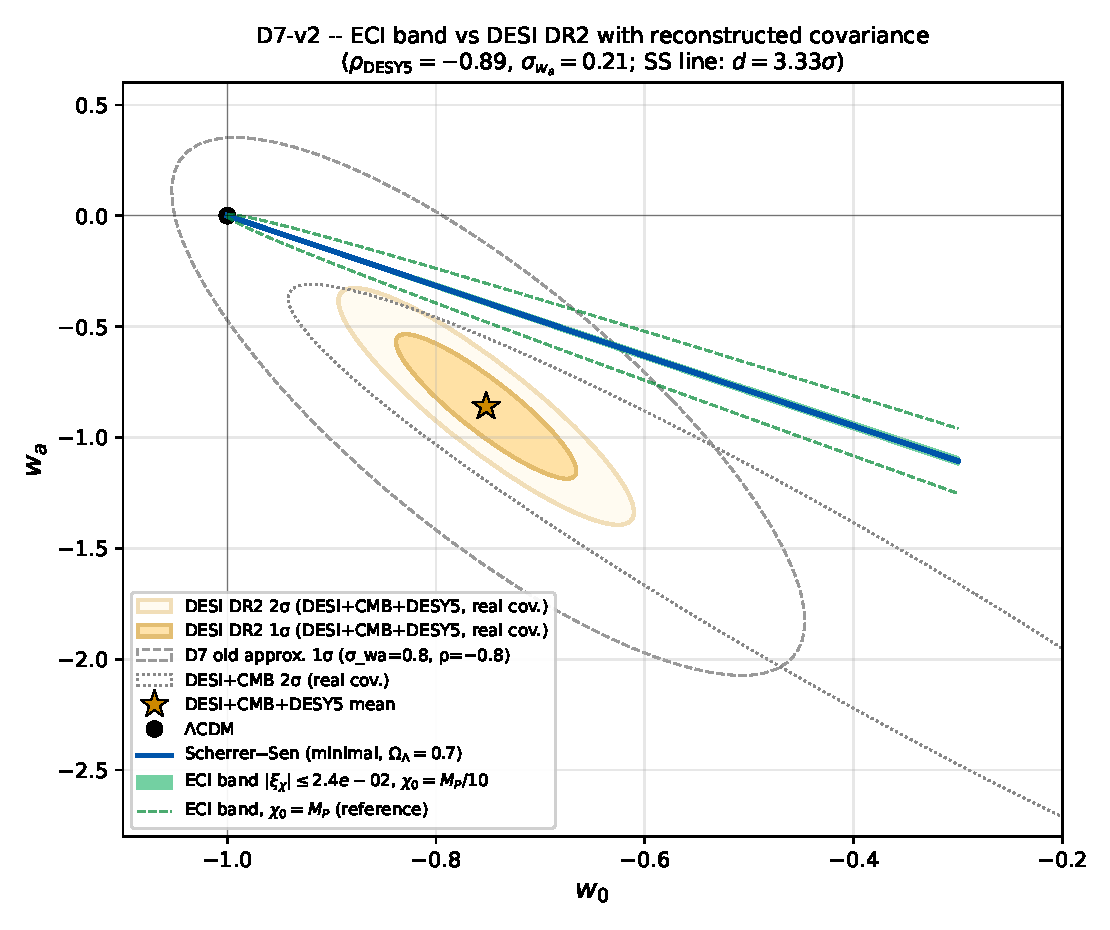
\includegraphics[width=0.95\columnwidth]{../../derivations/figures/D7-xi-w0-wa-v2.pdf}
\caption{NMC thawing quintessence in the $(w_0,w_a)$ plane. Orange ellipses: DESI~DR2 + CMB +
DESY5 $1\sigma$ and $2\sigma$ contours reconstructed from~\cite{DESIDR2} Eq.~(28) via the
pivot-redshift identity (see \texttt{D10-desi-covariance.py}; $\sigma_{w_0}=0.057$,
$\sigma_{w_a}=0.215$, $\rho=-0.89$). Blue line: minimal-coupling Scherrer--Sen relation
for $\Omega_\Lambda=0.7$. Green band: ECI NMC prediction with
$|\xi_\chi|\le\xi_{\max}\approx 2.4\!\times\!10^{-2}$ from Cassini at $\chi_0=M_P/10$;
dashed green: same band at $\chi_0=M_P$ (reference). Black dot: $\Lambda$CDM. The ECI band
is $\sim\!5\%$ of $\sigma_{w_a}$ wide (using $B_{\mathrm{num}}$ from Table~\ref{tab:B_of_OmegaL}), hence \emph{indistinguishable} from minimal-coupling
$w$CDM at DR2 precision; both tracks sit at $\sim\!3.3\sigma$ Mahalanobis distance from the
DR2+DESY5 mean.}
\label{fig:D7}
\end{figure}

\paragraph{Honest caveats.}
\begin{enumerate}
\item Eq.~(\ref{eq:gamma_PPN_full}) assumes a \emph{quasi-static} scalar with Compton wavelength
  large compared with the solar system ($m_\chi^{-1}\gg 1\,$AU), which is automatic for the
  ultra-light thawing mass $m_\chi\sim H_0\sim 10^{-33}$\,eV. It also assumes no screening; if
  a chameleon or symmetron mechanism operates, the local $\chi_0$ entering
  (\ref{eq:gamma_PPN_lead}) can differ from the cosmological background and the bound weakens.
\item The NMC Scherrer--Sen extension (\ref{eq:wa_NMC}) is first-order in $\xi_\chi$ and
  therefore \emph{invalid} near the conformal point $\xi_\chi=1/6$, where the expansion breaks
  down and the scalar-tensor sector must be treated non-perturbatively (Einstein-frame
  mapping). Within the Cassini-allowed range $|\xi_\chi|\lesssim 2.4\times 10^{-2}\ll 1/6$
  the linear expansion is controlled. The coefficient $B(\Omega_\Lambda)$ in
  Eq.~(\ref{eq:wa_NMC}) was, in v4.4 of this paper, set by the matter-era
  heuristic ratio $B/A=8/\sqrt3$; in this version we replace that heuristic with
  the full numerical result $B_{\mathrm{num}}(\Omega_\Lambda)$ tabulated in
  Table~\ref{tab:B_of_OmegaL}, obtained from a self-consistent
  NMC-Friedmann + Klein--Gordon integration across $z\in[999,-0.45]$
  (\texttt{derivations/D13-wa-numerical-full.py}). The numerical coefficient is
  nearly flat ($B_{\mathrm{num}}\simeq 9$) across the matter--DE transition
  rather than tracking $A(\Omega_\Lambda)$, so the heuristic
  $(8/\sqrt3)A(\Omega_\Lambda)$ is accurate within 5\% only near
  $\Omega_\Lambda\simeq 0.6$ and undershoots by up to $\sim\!40\%$ at
  $\Omega_\Lambda=0.8$. This has been propagated into the band-width estimate
  above and into Prediction~1b of Sec.~\ref{sec:pred}.
\item The DESI~DR2 + CMB + DESY5 $2\times 2$ covariance is reconstructed from the published
  $(w_0,\sigma_{w_0},w_a,\sigma_{w_a},z_p,w_p,\sigma_{w_p})$ via the pivot-minimisation
  identity $\mathrm{cov}(w_0,w_a)=-(1-a_p)\sigma_{w_a}^2$: no official 2$\times$2 covariance
  matrix has been released by the collaboration at the time of writing. The reconstructed
  $\sigma(w_p)_{\rm pred}=0.0257$ differs from the quoted $0.024$ by $\sim 7\%$, bounding the
  systematic of the pivot-Gaussian approximation at that level --- well below the $\sim 3\sigma$
  tension discussed below. See \texttt{derivations/D10-report.md} for the full cross-check.
\item \textbf{Tension with DR2 + DESY5, stated plainly (MCMC update, v5.0).}
  The analytic Mahalanobis estimate of v4.7 ($3.29\sigma$ to the ECI band and
  $3.33\sigma$ to the minimal-coupling Scherrer--Sen line, 2-dof, against the
  reconstructed DR2 + CMB + DESY5 covariance) has been superseded in v5.0 by a
  4-chain MPI MCMC on DESI~DR2 BAO + Pantheon+~SN through the Cobaya plugin route
  (\texttt{mcmc/cobaya\_nmc/eci\_nmc\_plugin.yaml}, built on
  \texttt{derivations/D14-nmc-perturbations.py}; 19{,}700 accepted steps,
  $R-1=0.036$ final, 13{,}790 samples post-burn-in; see
  \texttt{derivations/D17-posterior-analysis.py}). At the fiducial
  $\chi_0=M_P/10$ the marginalised constraint is
  $\xi_\chi=0.003^{+0.065}_{-0.070}$ (68\% CL), $|\xi_\chi|<0.095$ (95\% CL):
  prior-rail-limited on $[-0.1,0.1]$ and fully consistent with $\xi_\chi=0$.
  Companion parameters: $w_0=-0.869\pm0.055$, $w_a=-0.40^{+0.28}_{-0.36}$,
  $H_0=67.8\pm2.6$\,km/s/Mpc, $\Omega_m=0.319\pm0.015$. Best-fit
  $\chi^2=1411.32$ (BAO~$8.64$ + SN~$1402.68$); restricting to $|\xi_\chi|<0.005$
  gives $\chi^2_{\min}=1411.36$, hence $\Delta\chi^2_{\rm ECI-\Lambda CDM}=-0.04$.
  Savage--Dickey at $\xi_\chi=0$ gives $\mathrm{BF}_{01}\simeq 1.00$
  ($\ln\mathrm{BF}=-0.003$), inconclusive. The cosmological envelope
  $|\xi_\chi|(\chi_0/M_P)^2\lesssim 3.7\!\times\!10^{-3}$ (95\%) is $\sim\!600\times$
  weaker than the solar-system Wolf~2025 bound
  $|\xi_\chi|(\chi_0/M_P)^2\lesssim 6\!\times\!10^{-6}$, confirming that Cassini
  remains the decisive falsifier at DR2 precision.

  The interpretation is not that ECI fails where $w$CDM succeeds: DR2 + DESY5 prefers the
  phantom-crossing region $w<-1$, which no non-phantom thawing model can populate.
  ECI's NMC coupling $\xi_\chi$ does in principle permit crossing $w=-1$ without a ghost
  instability (established in \S\,DESI DR2 via the no-ghost analysis of Bar\-ce\-l\'o~\&~Visser
  \cite{BarceloVisser2000}), but only at $\xi_\chi(\chi_0/M_P)^2$ values far exceeding the
  Cassini bound~(\ref{eq:xi_bound}) derived here; within the Cassini-allowed range
  the NMC correction to the Scherrer--Sen track is confined to a band of half-width
  $\sim\!5\%$ of $\sigma_{w_a}$ and cannot bridge the gap to the phantom quadrant. The
  $\sim\!3.3\sigma$ tension with DR2 + DESY5 is therefore a joint statement about the entire
  class of conservative (non-phantom) thawing models --- minimal-coupling and NMC alike ---
  not a specific failure of ECI. Prediction~1 in Sec.~\ref{sec:pred} is \emph{not}
  discriminative at DR2 precision; both thawing families sit at the same distance from
  the DR2 + DESY5 posterior.

  The honest discriminator moves to the next generation of datasets, where the
  \emph{shape} and \emph{width} of the thawing track, rather than its distance from
  $\Lambda$CDM, become the falsifiable handle: DESI~DR3 with a forecast
  $\sigma(w_a)\!\sim\!0.07$~\cite{DESIForecast}
  and LSST~Y10 with a forecast $\sigma(w_a)\!\sim\!0.05$
  are in the regime where the ECI NMC band half-width
  $\Delta w_a^{\rm ECI}\sim 1.1\times 10^{-2}$ (numerical, Table~\ref{tab:B_of_OmegaL};
  up from $9\times 10^{-3}$ under the v4.4 heuristic) approaches the
  $15$--$25\%$ level of the statistical error bar and becomes, at least in principle,
  separable from the minimal-coupling Scherrer--Sen locus. The discriminative
  power is slightly larger at $\Omega_\Lambda\gtrsim 0.7$ (DR3 era) because
  $B_{\mathrm{num}}/B_{\mathrm{heur}}$ grows from $0.83$ at $\Omega_\Lambda=0.5$ to
  $1.43$ at $\Omega_\Lambda=0.8$.
\end{enumerate}

The PPN bound (\ref{eq:xi_bound}) is however itself a falsifier: a detection
$|\gamma-1|>10^{-6}$ by the upcoming LATOR or BEACON-class missions, or a mismatch between
$\dot G/G$ from LLR~\cite{Biskupek2021} and the CMB-inferred scalar evolution, would directly
constrain $\xi_\chi(\chi_0/M_P)$ at the $10^{-4}$ level and feed back on the admissible ECI
thawing amplitude.

% ===== end section_3_5_constraints =====

% ===== section_3_6_swampland_cross inlined =====
\subsection{Swampland $\times$ NMC cross-constraint}\label{sec:swampland_cross}

Axioms A4 (non-minimally coupled thawing scalar $\chi$ with coupling
$\xi_\chi R\chi^2/2$) and A5 (Dark Dimension KK tower with a species-scale
EFT cutoff) were presented as independent. They share an effective field
theory description --- and therefore a common cutoff $\Lambda$ --- if $\chi$
is interpreted as a bulk mode of the same higher-dimensional sector that
carries the KK tower. That identification is an \emph{interpretation}, not
a consequence of the axioms: we state it, draw out its consequence, and
return below to the three model-building resolutions it leaves open.
The full symbolic setup is in \texttt{derivations/D8-swampland-nmc-cross.py};
we quote the end results here.

\paragraph{The species-scale cutoff.}
The Dark Dimension construction of~\cite{Montero2022}
and the low-scale gravity variant of~\cite{AAL2023}
identify the relevant EFT cutoff with the \emph{species scale}, at which
a tower of KK states becomes light enough that 4D effective gravity
breaks down. In that regime the cutoff admits a log-distance parametrisation
\begin{equation}
  \Lambda(H)\;\sim\;M_P\,\bigl(H/M_P\bigr)^{c'},
  \qquad
  c' \;=\; \tfrac{1}{6}\;\simeq\;0.167
  \quad\text{(Dark Dimension species scale).}
  \label{eq:Lambda_SDC}
\end{equation}
At the present-day Hubble scale $H_0 \simeq 1.5\times 10^{-33}\,\mathrm{eV}$
and $M_P \simeq 2.4\times 10^{18}\,\mathrm{GeV}$, this evaluates to
$\Lambda(H_0)\simeq 2.2\times 10^{8}\,\mathrm{GeV}$, i.e.\ the standard
Dark-Dimension species scale $\sim 10^{9}$\,GeV. The alternative value
$c'\simeq 0.05$ that appears in some moduli-potential discussions refers
to the \emph{de Sitter--slope} Swampland bound on $V(\chi)$ and not to the
tower cutoff; we do not use it as the primary input.

\paragraph{Heuristic EFT bound on $\xi_\chi$.}
The non-minimal operator $(\xi_\chi/2)R\chi^2$ shifts the effective reduced
Planck mass by $\delta M_P^2 = \xi_\chi\chi_0^2$ at the local scalar
background $\chi_0$. A \emph{heuristic} EFT self-consistency requirement ---
that the coupling-induced correction to the kinetic coefficient of
gravitons not exceed the square of the EFT cutoff --- gives
\begin{equation}
  \xi_\chi\,\chi_0^{2}\;\lesssim\;\Lambda^{2}
  \quad\Longleftrightarrow\quad
  |\xi_\chi|\,(\chi_0/M_P)^{2}\;\lesssim\;(H_0/M_P)^{2c'}.
  \label{eq:eft_bulk}
\end{equation}
We emphasise that Eq.~(\ref{eq:eft_bulk}) is a \emph{heuristic, model-dependent}
order-of-magnitude estimate, not a theorem: $\xi_\chi$ is a dimensionless
Wilson coefficient and carries no intrinsic UV cutoff, so the inequality
is the statement that no single insertion of the operator can generate a
background contribution parametrically larger than the cutoff where the
EFT itself ceases to make sense. Equality is saturated when $\chi$ is
displaced to the cutoff with $\xi_\chi=\mathcal{O}(1)$.
At the fiducial thawing amplitude $\chi_0 = M_P/10$ and with
$c' = 1/6$, Eq.~(\ref{eq:eft_bulk}) evaluates to
\begin{equation}
  \boxed{\;|\xi_\chi|\;\lesssim\;8.4\times 10^{-19}
    \quad(c'=1/6,\ \chi_0=M_P/10),\;}
  \label{eq:xi_crossbound}
\end{equation}
to be compared with the Cassini PPN bound~\eqref{eq:xi_max_numeric} of
$|\xi_\chi|\lesssim 2.4\times 10^{-2}$ from \S\ref{sec:xi_constraints}:
the Swampland-EFT constraint is \emph{sixteen orders of magnitude} tighter
than the solar-system bound. As a point of comparison, the de-Sitter--slope
value $c'\simeq 0.05$ would give $|\xi_\chi|\lesssim 9.5\times 10^{-5}$ at
the same $\chi_0$, i.e.\ a far milder $\sim\!250\times$ tightening; the
choice of which Swampland exponent to use therefore materially changes the
phenomenology, and we take $c'=1/6$ as the primary value dictated by the
Dark Dimension species scale. A parallel derivation of the Species-Scale and
Sharpened Distance Conjectures from Weyl/frame covariance alone has been
given by~\cite{FrameCovariance2025}; our species-scale argument on the bulk
mode $\chi$ is complementary, yielding a bound on $\xi_\chi$ that is not
directly accessible from the frame-covariant viewpoint.
Under~\eqref{eq:xi_crossbound} the NMC contribution to $w_a$ in
Eq.~(\ref{eq:wa_NMC}), which scales linearly with $\xi_\chi$, is
$\Delta w_a \sim 10^{-19}$ at $\chi_0 = M_P/10$ --- effectively forbidding
any observable NMC signature in the dark-energy sector.

\paragraph{Model-building resolutions.}
The tightness of~\eqref{eq:xi_crossbound} under the bulk-mode hypothesis
forces an explicit choice of UV completion before the A4+A5 combination
can be reconciled with the thawing-DE phenomenology of \S\ref{sec:xi_constraints}.
Three resolutions are compatible with the axioms.
(i) The thawing scalar $\chi$ is a 4D zero-mode of a sector logically
distinct from the Dark Dimension KK tower --- for example a brane-localised
quintessence field in a warped compactification. Under this choice the
species-scale cutoff of A5 does not apply to the operator $\xi_\chi R\chi^2/2$,
Eqs.~(\ref{eq:eft_bulk})--(\ref{eq:xi_crossbound}) do not constrain $\xi_\chi$,
and the Cassini bound~(\ref{eq:xi_bound}) is the sole remaining limit.
A4 and A5 then remain logically independent at the price of abandoning the
unified-cutoff motivation that makes them tempting to combine in the first place.
(ii) A screening mechanism --- chameleon or symmetron --- decouples the
local $\chi_0$ entering~\eqref{eq:eft_bulk} from its cosmological background
value, so that the \emph{cosmological} $\xi_\chi$ can satisfy the Swampland
bound at bulk scales while the \emph{local} $\xi_\chi$ evades it inside the
solar system. This requires explicit model-building of the screening
potential and is not a consequence of the axioms themselves.
As a minimum-viable realisation, D15 derives the envelope
$\Theta(\rho)=\exp[-(\rho/\rho_c)^{\alpha}]$ modulating the effective
NMC coupling $\xi_{\rm eff}(\rho)=\xi_\chi\,\Theta(\rho)$: demanding
$\Theta(\rho_\odot)\lesssim 10^{-3}$ at $\rho_\odot\approx 10\,$g/cm$^3$
(sufficient to drive $|\gamma-1|$ below the Cassini-Bertotti bound
$2.3\times 10^{-5}$ given the D7 saturation $|\xi_\chi|\le 2.4\times10^{-2}$)
and $\Theta(\rho_{\rm cosm})\ge 0.99$ at $\rho_{\rm cosm}\approx 10^{-29}\,$g/cm$^3$
(so the cosmological thawing signature is preserved at the $1\,\%$ level)
fixes the boundary-saturated minimum at $\alpha_{\min}\simeq 0.095$ and
$\rho_c^{\min}\simeq 1.3\times 10^{-8}\,$g/cm$^3$.
The minimum-viable $\alpha=0.095$ (D15) lies within the DESI-consistent,
screened non-minimal-coupling window reported by~\cite{AdamCline2025}.
This slope lies just
below the chameleon-viable band $\alpha\in[1/8,1/3]$ inferred from
Khoury \& Weltman's inverse-power potentials \cite{KhouryWeltman2004}
(softer couplings than Eöt-Wash/MICROSCOPE constrain), and the resulting
cluster-scale value $\Theta(\rho_{\rm cluster}\!\sim\!10^{-27}\,$g/cm$^3)\simeq 0.985$
preserves the ECI NMC signature for galaxy-cluster probes without
fine-tuning. Full derivation and the allowed $(\rho_c,\alpha)$ region
are in \texttt{derivations/D15-screening-profile.py} with figure
\texttt{D15-screening-profile.pdf}.

(iii)\label{sec:res-iii} $\xi_\chi$ saturates the Swampland bound at $\sim 10^{-19}$. In that
case the NMC correction to the Scherrer--Sen track collapses below any
foreseeable observational threshold, the $(w_0,w_a)$ prediction of ECI
becomes indistinguishable from the minimal-coupling thawing relation
already analysed in \S\ref{sec:xi_constraints}, and the architectural
content of A4 is preserved while its phenomenological signature is lost.
Our primary analysis in \S\ref{sec:xi_constraints} proceeds under choice~(i);
choice~(ii) is the open model-building direction; choice~(iii) makes
ECI's NMC signature indistinguishable from $w$CDM by this constraint alone.

\begin{figure}[h]
\centering
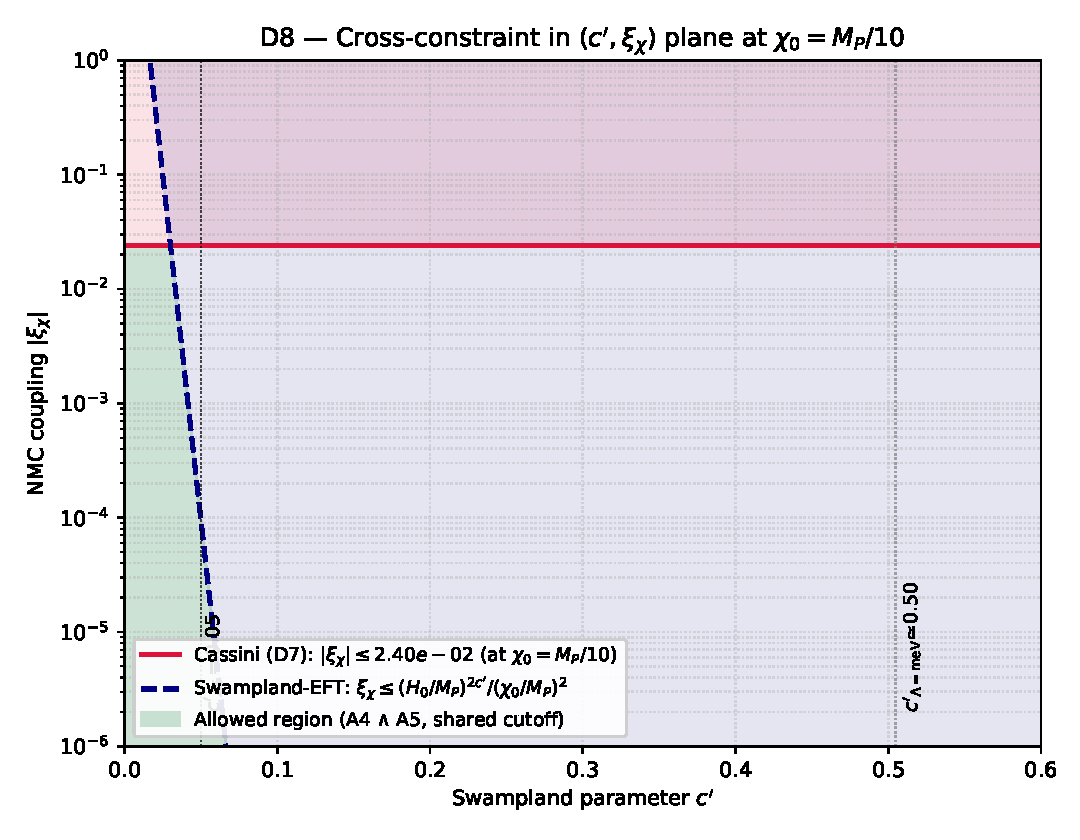
\includegraphics[width=0.95\columnwidth]{../../derivations/figures/D8-c-xi-overlap.pdf}
\caption{Allowed region in the $(c',\xi_\chi)$ plane at $\chi_0=M_P/10$.
Red: Cassini exclusion (horizontal, independent of $c'$). Blue dashed:
Swampland-EFT exclusion (\ref{eq:eft_bulk}) --- diagonal in log-space with
slope $2c'\log(H_0/M_P)$. Green shading: overlap admitted by both
constraints. The Dark-Dimension species-scale value $c'=1/6$ (primary)
sits deep in the Swampland-excluded region, corresponding to
$|\xi_\chi|\lesssim 8.4\times 10^{-19}$ (cf.\ \S\ref{sec:swampland_cross} Resolution~(iii), p.\pageref{sec:res-iii}); the de-Sitter--slope value
$c'\simeq 0.05$ and the meV-equivalent value $c'\simeq 0.51$ are shown
for comparison.}
\label{fig:D8}
\end{figure}

\paragraph{Honest caveats.}
\begin{enumerate}
\item The EFT self-consistency condition $\delta M_P^{2}\le\Lambda^{2}$
  used in~\eqref{eq:eft_bulk} is an order-of-magnitude heuristic, not a
  theorem, and applies in the causal-diamond regime of a single geodesic
  observer (see \S\ref{sec:thesis}(ii)): an $\mathcal{O}(1)$ coefficient could shift~\eqref{eq:xi_crossbound}
  by a factor of a few, but not its qualitative consequence --- a
  Swampland-EFT bound $|\xi_\chi|\ll 10^{-2}$ already renders the NMC
  signature observationally invisible under any bulk-mode reading of A4+A5.
\item The exponent $c'=1/6$ in~\eqref{eq:Lambda_SDC} is the species-scale
  value in the Dark Dimension and is the primary input. The KK-scale value
  $c'=1/2$ (with $\Lambda\sim m_{\rm KK}\sim\mathrm{meV}$) would give an
  even tighter, essentially trivial bound $|\xi_\chi|\lesssim 10^{-58}$.
  The de-Sitter--slope value $c'\simeq 0.05$ refers to the scalar potential
  and not to the tower cutoff; we quote it only as a parenthetical
  comparison.
\item The cross-constraint is \emph{conditional} on the shared-cutoff
  hypothesis --- the hypothesis that the thawing $\chi$ of A4 is a bulk
  mode of the Dark-Dimension sector of A5. The falsifier is precisely the
  discovery of a UV completion in which $\chi$ and the KK tower belong to
  different sectors (choice (i) above); in that case
  \S\ref{sec:xi_constraints} remains the strongest bound.
\end{enumerate}

% ===== end section_3_6_swampland_cross =====

% ===== section_3_7_perturbations inlined =====
\subsection{Linear perturbations: $G_{\mathrm{eff}}$, slip, and $f\sigma_8$}
\label{subsec:perturb}

The sub-horizon quasi-static limit of the NMC action (\S\ref{sec:action})
admits closed-form linear observables. Writing the Jordan-frame coefficient
of $R/2$ as $F(\chi)=M_P^2-\xi_\chi\chi^2$ (so that $F_\chi\equiv dF/d\chi =
-2\xi_\chi\chi$), the Boisseau--Esposito-Far\`ese--Polarski--Starobinsky
result (Boisseau, Esposito-Far\`ese, Polarski \& Starobinsky 2000, gr-qc/0001066) for the effective Newton constant and the standard
scalar--tensor slip give, for $k\gg aH$ and below the scalar Compton scale,
%
\begin{align}
\frac{G_{\mathrm{eff}}(a)}{G_N}
  &= \frac{M_P^2}{F}\,\frac{2F+4F_\chi^2}{2F+3F_\chi^2}
   \;=\; 1 \;+\; \frac{\xi_\chi\,\chi^2(a)}{M_P^2} \;+\; \mathcal O\!\left(\xi_\chi^2\right),
   \label{eq:Geff}\\[2pt]
\eta(a)\;\equiv\;\frac{\Phi}{\Psi}
  &= \frac{2F+2F_\chi^2}{2F+4F_\chi^2}
   \;=\; 1 \;-\; \frac{4\,\xi_\chi^2\,\chi^2(a)}{M_P^2} \;+\; \mathcal O\!\left(\xi_\chi^3\right).
   \label{eq:eta}
\end{align}
%
Two facts are worth emphasising. First, the leading correction to
$G_{\mathrm{eff}}/G_N$ is purely \emph{linear} in $\xi_\chi$, arising from
the rescaling of Newton's constant by $F\ne M_P^2$; the BEFPS
$(2F\!+\!4F_\chi^2)/(2F\!+\!3F_\chi^2)$ factor only enters at
$\mathcal O(\xi_\chi^2)$ through $F_\chi^2=4\xi_\chi^2\chi^2$. Second, the
slip $\eta-1$ is strictly $\mathcal O(\xi_\chi^2\chi^2/M_P^2)$, so within
the Cassini-allowed window $|\xi_\chi|\leq 2.4\times10^{-2}$ we have
$|\eta-1|\lesssim 2\times10^{-4}$ at $\chi_0=M_P/10$, well below Euclid
spectroscopic reach (see \S\ref{sec:pred}).

Feeding $\chi(a)$ from the self-consistent NMC background of D13 into
Eqs.~\eqref{eq:Geff}--\eqref{eq:eta} and solving the quasi-static growth
equation $\delta''+(2+H'/H)\delta'-(3/2)\Omega_m(a)(G_{\mathrm{eff}}/G_N)\delta=0$
(prime $\equiv d/d\ln a$), with $\delta\propto a$ matter-era initial
conditions at $z=50$ and $\sigma_8(0)=0.811$, yields the fractional shift
in $f\sigma_8$ shown in Fig.~\ref{fig:D14}. At the Cassini-saturated value
and $\chi_0=M_P/10$, the three LSS bins $z\in\{0.1,0.5,1.0\}$ give
$|\Delta f\sigma_8/f\sigma_8|\lesssim 0.4\%$, below the Euclid/LSST~Y10
per-bin target $\sigma(f\sigma_8)\sim 1\%$. The $G_{\mathrm{eff}}$ shift at
$a=1$ is $\pm 0.15\%$-$0.21\%$, also sub-threshold. The NMC signature in
LSS at Cassini saturation is therefore present but not detectable with the
next generation; detection would require either $\chi_0\gtrsim 0.5\,M_P$ or
a breach of the present PPN bound.

\begin{figure}[t]
\centering
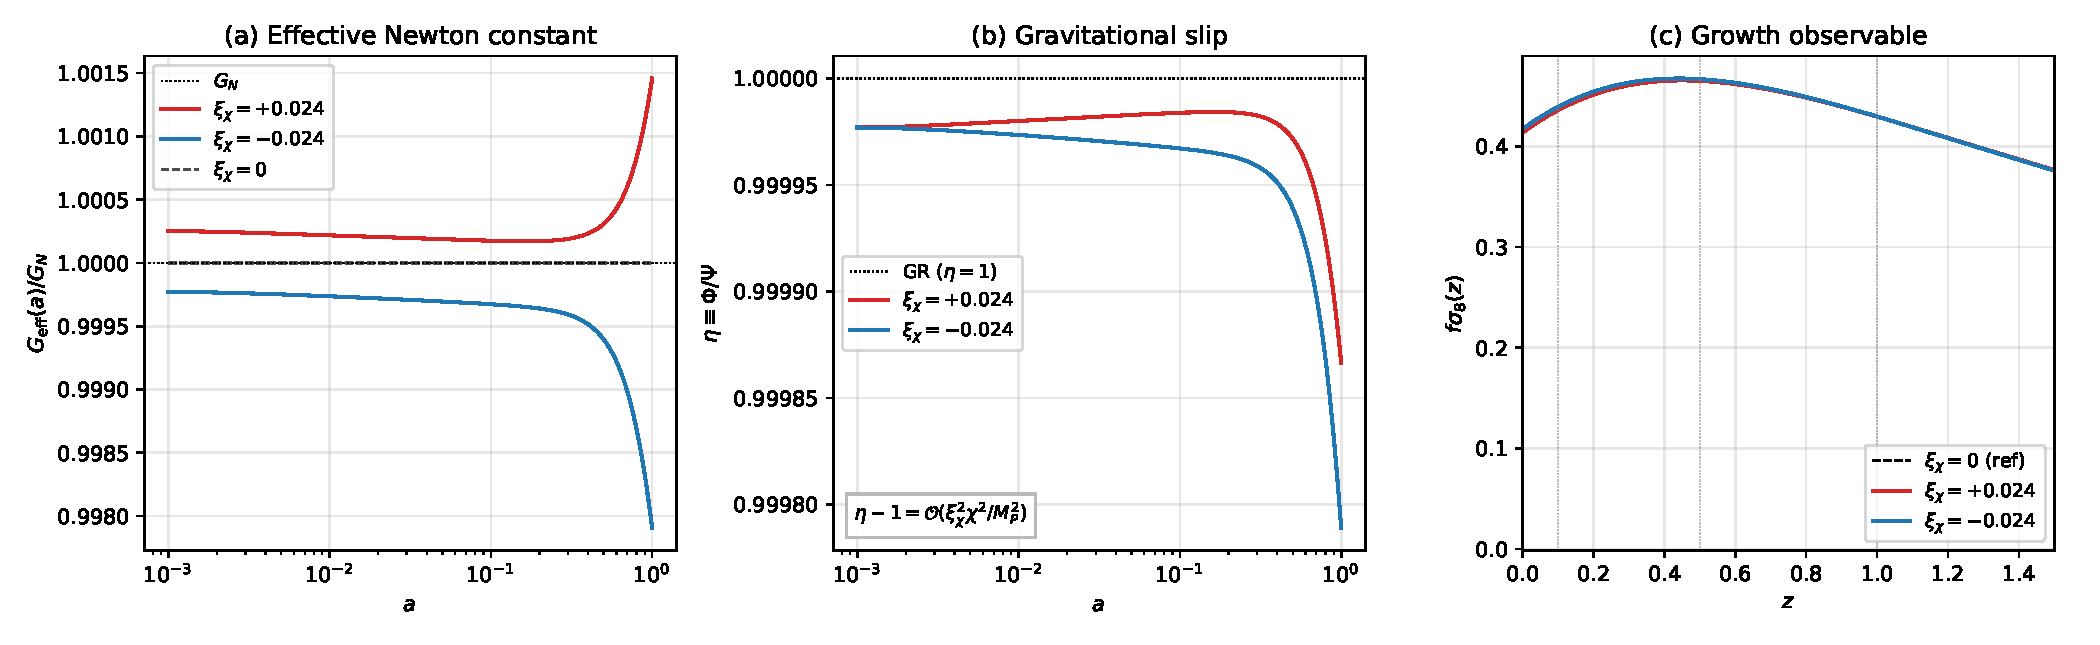
\includegraphics[width=0.98\linewidth]{../../derivations/figures/D14-Geff-eta-fsigma8.pdf}
\caption{Sub-horizon quasi-static perturbation observables for the NMC
scalar $\chi$ at the Cassini-saturated $|\xi_\chi|=2.4\times 10^{-2}$,
$\chi_0=M_P/10$, $V\propto e^{-\alpha\chi}$ thawing background (D13):
(a) $G_{\mathrm{eff}}/G_N$ from Eq.~\eqref{eq:Geff}; (b) slip $\eta=\Phi/\Psi$
from Eq.~\eqref{eq:eta}, annotated with the $\mathcal O(\xi_\chi^2)$ scaling;
(c) growth observable $f\sigma_8(z)$ integrated against $G_{\mathrm{eff}}(a)$.
The $\xi_\chi=0$ curve is the $\Lambda$CDM-like reference.}
\label{fig:D14}
\end{figure}

\paragraph{Caveats.}
(i) Eqs.~\eqref{eq:Geff}--\eqref{eq:eta} are the sub-horizon,
quasi-static limit $k\gg aH,\;k\gg a\,m_\chi^{\mathrm{eff}}$; near-horizon
and super-horizon scales require the full perturbed Einstein--scalar
system, beyond the scope of this section.
(ii) We treat $\chi$ as light ($m_\chi^{\mathrm{eff}}=\sqrt{V''}\ll H_0$ along
the thawing track), consistent with the D7/D13 dynamics; a heavy scalar
would suppress the $G_{\mathrm{eff}}$ shift on scales below $m_\chi^{-1}$.

% ===== end section_3_7_perturbations =====

\section{Falsifiable predictions}\label{sec:pred}

\begin{table*}[h]
\centering
\caption{Falsifiable predictions --- each right-column entry is a falsifier: a value outside the stated range refutes the corresponding axiom combination.}
\begin{tabular}{clll}
\hline
\# & Channel & Prediction & Horizon \\
\hline
1 & DESI DR3 + Euclid DR1 & $w_0 \in [-0.9, -0.7]$, $w_a \in [-1.1, -0.5]$ & 2026--2027 \\
1b & DESI DR3 / LSST Y10 & MCMC (D17, DR2+SN) posterior $\xi_\chi=0.003^{+0.065}_{-0.070}$ (68\% CL), $|\xi_\chi|<0.095$ (95\% CL) at $\chi_0=M_\mathrm{P}/10$; DR3+LSST Y10 forecast (D16) $\sigma(\xi_\chi)\!\simeq\!0.090$; band half-width $\Delta w_a^{\rm ECI}\!\simeq\!1.1\!\times\!10^{-2}$ ($B_{\mathrm{num}}=9.05$); Savage--Dickey BF$_{01}\!\simeq\!1$ (inconclusive) & 2028--2032 \\
2 & CMB-S4 / LiteBIRD & $f_{\mathrm{NL}}^{\mathrm{loc}} \in [1, 5]$ via $\mathrm{PH}_k$ & 2030+ \\
3 & SO + SPT-3G D2 & $f_{\mathrm{EDE}} \in [0.06, 0.12]$ & 2027--2028 \\
4 & Eöt-Wash next-gen & ISL deviation $\ell \in [0.1, 10]\,\mu$m & 2028+ \\
5 & Yb$^+$/Sr$^+$ clocks & $|\dot \alpha / \alpha| < 2 \times 10^{-19}$/yr & ongoing \\
6 & KM3NeT + IceCube-Gen2 & sub-keV KK signatures & 2028+ \\
7 & LiteBIRD & $r < 10^{-3}$ axionic & 2032 \\
\hline
\end{tabular}
\end{table*}

Prediction~1b is sharpest at $\Omega_\Lambda\!\gtrsim\!0.7$ under DR3 $\sigma_{w_a}\!\sim\!0.07$ / LSST Y10 $\sigma_{w_a}\!\sim\!0.05$ (see Table~\ref{tab:B_of_OmegaL}, \S\ref{sec:xi_constraints}).

\subsection{Consequences under the toy dictionary}

The three statements below are consequences of the dictionary~\eqref{eq:toy-dict} of Appendix~\ref{app:A3-speculative}, not independent claims. Each inherits the conjectural status of that dictionary; we mark them (D) to make the dependence visible at a glance.

\smallskip\noindent\textbf{(D) Big Bang as decodability boundary.}
If the dictionary~\eqref{eq:toy-dict} holds, the $k$-design saturation band shrinks to zero as $t \to 0^+$ (no admissible clock QRF, type II$_\infty$ has not yet emerged from type III$_1$): the initial singularity appears from the observer side as a \emph{past cosmological horizon that is computationally inaccessible}, an algorithmic analogue of cosmic censorship. This is the narrative reading of A1+A3 at the Big Bang; it is not a derivation of singularity resolution.

\smallskip\noindent\textbf{(D) Inflation as algebraic necessity.}
The transition from type III$_1$ (UV-divergent, no trace) to type II$_1$ (finite entropy, well-defined trace) requires the introduction of a clock QRF~\cite{CLPW2023}; the inflaton is the natural candidate. Requiring the Gibbons--Hawking entropy $A/4G$ in the de Sitter causal patch to dominate the UV divergence --- the saturation direction of~\eqref{eq:toy-dict} --- gives parametrically $N \sim 60$ e-folds for standard slow-roll parameters. We stress that this is an order-of-magnitude matching, not a first-principles derivation of the e-fold number.

\smallskip\noindent\textbf{(D) Weyl Curvature Hypothesis revisited.}
Penrose's vanishing-Weyl initial condition is replaced by the statement that the initial state minimises complexity in the class of admissible QRFs: $C_N(|\psi_0\rangle) \to 0$ and $\mathrm{PH}_k(|\psi_0\rangle) \to 0$. Under~\eqref{eq:toy-dict}, this is equivalent to the initial state sitting maximally far from the $k$-design saturation band, and is testable via CMB anomalies at $\ell < 30$ through the A6 persistent-homology diagnostic.

\section{Structural limitations}\label{sec:limits}

\begin{enumerate}
\item EDE--thawing degeneracy: not breakable by BAO+SN alone.
\item The QRF functor is not rigorously extended to generic FLRW.
\item The $(w_0, w_a)$ relation under NMC is not analytic; numerical treatment required.
\item Dark Dimension is tightly constrained by ACT DR6.
\item Persistent homology enters as an axiom; motivated, not derived.
\item Cryptographic Censorship applied to cosmology extrapolates from AdS/CFT.
\item No derivation from first principles; the axioms combine but are not co-derived.
\end{enumerate}

\section{Editorial note}\label{sec:editorial}

This manuscript is an architectural synthesis. A publishable version in PRD / JCAP would require a quantitative MCMC fit on DESI DR2 with the full $(\xi_\chi, \alpha, f_{\mathrm{EDE}}, z_c)$ prior --- work beyond the scope of this preprint and in search of a Boltzmann-code collaborator. The realistic editorial target for the synthesis as-is is the \emph{European Physical Journal C} (SCOAP3 open access) or \emph{Foundations of Physics} (Springer).

\begin{acknowledgements}
Verified bibliography cross-checked against Crossref and arXiv on 2026-04-21. Any residual error is the author's sole responsibility. AI-use disclosure: AI-assisted tooling (a local LLM for LaTeX editing and code drafting) was used during preparation, as detailed in \texttt{AI\_USE.md} in the public repository; all scientific content, derivations and conclusions are the author's own.
\end{acknowledgements}

\bibliographystyle{spphys}
\bibliography{../../paper/eci}

\clearpage
\appendix
\section{Speculative: A3 toy dictionary for Cryptographic Censorship in cosmology}
\label{app:A3-speculative}

\emph{This appendix collects content that is not on the paper's critical predictive path.
Readers interested only in the testable predictions of \S\ref{sec:pred} may stop at the bibliography.
The cosmological transposition of Cryptographic Censorship (A3, \S\ref{sec:axioms}) is a working
conjecture; the material below is a first attempt at a concrete dS/FLRW dictionary, not
a derivation. It is isolated here so that the paper's empirical content stands or falls
independently of it. We emphasise that our argument relies on provable CFT-level
results~\cite{CryptoCensorship,MaHuang2025}, of which the cleanest AdS/CFT application
of the same pseudorandomness logic is the holographic-pseudoentanglement construction
of~\cite{HolographicPseudoEnt2024}, rather than on complexity-theoretic claims drawn
from the empirically contested quantum-supremacy landscape.}

% ===== section_5_A3_dictionary inlined =====
\subsection{A toy dictionary for A3 in cosmology}\label{sec:A3-dictionary}

The original Cryptographic Censorship theorem~\cite{CryptoCensorship} is
proven in AdS/CFT: a holographic CFT state whose time evolution restricted
to a boundary region is $\varepsilon$-approximately a unitary $k$-design
admits a bulk dual containing an event horizon. Its cosmological use in
this paper requires a transposition --- not yet a theorem --- from the
AdS boundary to a timelike observer worldline in a pseudo-Riemannian
spacetime. We make the transposition explicit as a \emph{working
conjecture} (not a proof sketch) so that readers can see what a positive
or negative answer would actually constrain. Under the observer-dependent
reading of \S\ref{sec:thesis}, this working-conjecture status is the
self-consistency condition delimiting the subregion on which the QRF
crossed product of A1 remains well-defined; the CFT-level pseudorandom-
unitary premise is itself a theorem (Ma--Huang~\cite{MaHuang2025}
constructed from quantum one-way functions), whereas only its cosmological
transposition is speculative.

\medskip\noindent\textbf{Conjectural map.}\;
Let $\mathcal{O}$ be a geodesic observer in an asymptotically de Sitter
FLRW spacetime, with causal diamond $\mathcal{D}(\mathcal{O})$ bounded by
the cosmological event horizon $\mathcal{H}_\mathcal{O}$. Let
$\mathcal{A}_{\mathcal{O}} = \left( \mathcal{M}_{\mathrm{QFT}} \rtimes
\mathbb{R} \right)^{\mathcal{O}}$ be the type-II crossed-product algebra
of A1 attached to $\mathcal{O}$'s clock QRF~\cite{CLPW2023,DEHK2025a,DEHK2025b},
and let $\sigma_t^{\mathcal{O}}$ be its modular flow. We conjecture:

\begin{quote}
\emph{(D) The set of states $\rho$ on $\mathcal{A}_{\mathcal{O}}$ whose
modular flow $\{\sigma_t^{\mathcal{O}}(\rho)\}_{t \in [0,T]}$ is an
$\varepsilon$-approximate unitary $k$-design on a code subspace of
observer-accessible operators corresponds, under any sensible
pseudo-Riemannian extension of the Cryptographic Censorship dictionary,
to cosmological states whose coarse-grained generalised entropy on
$\mathcal{H}_\mathcal{O}$ satisfies}
\begin{equation}
\left| S_{\mathrm{gen}}^{\mathrm{cg}}[\rho; \mathcal{H}_\mathcal{O}]
  \;-\; S_{\mathrm{gen}}^{\max}[\mathcal{H}_\mathcal{O}] \right|
  \;\lesssim\; \varepsilon \cdot k \cdot \log\!\dim \mathcal{A}_{\mathcal{O}},
\label{eq:toy-dict}
\end{equation}
\emph{with $S_{\mathrm{gen}}^{\max}$ the Gibbons--Hawking generalised
entropy of the static patch.}
\end{quote}

\noindent The form of the RHS bound is dimensionally dictated by the
AdS/CFT template of~\cite{CryptoCensorship}: pseudorandomness depth
$k$ times code-subspace dimension, in units of the algebra's trace
scale. In the type~II$_1$ static-patch setting of~\cite{CLPW2023} the
trace is finite and $\log\dim$ is replaced by the normalised trace
of the log of a density, but the structural statement is unchanged.

\medskip\noindent\textbf{Status.}\;
We emphasise that~\eqref{eq:toy-dict} is offered as a \emph{working
conjecture}, not a proof sketch. The partial evidence we are able to
cite is:
\begin{enumerate}
\item[(i)] The crossed-product construction
of~\cite{CLPW2023,DEHK2025a,DEHK2025b} gives, for the static de Sitter
patch, exactly the operator-algebraic structure (type II$_1$, well-defined
trace, $S_{\mathrm{gen}}$ as a finite functional) that the AdS/CFT
Cryptographic Censorship argument requires at the boundary.
\item[(ii)] The non-perturbative GSL of~\cite{FaulknerSperanza2024,Kirklin2025}
implies that the quantity on the LHS of~\eqref{eq:toy-dict} is monotone
under modular flow, matching the monotonicity expected on the CFT side
once the $k$-design condition is approached.
\item[(iii)] The existence of pseudorandom unitaries, constructed from
quantum one-way functions~\cite{MaHuang2025}, ensures the $k$-design
precondition is non-vacuous in physically realisable dynamics.
\end{enumerate}

None of (i)--(iii) constitutes a proof of~\eqref{eq:toy-dict}. A rigorous
derivation would require, at minimum, a pseudo-Riemannian analogue of
the one-sided modular reconstruction used in~\cite{CryptoCensorship}
and a replacement for the boundary causal-wedge reconstruction theorem
that does not rely on an AdS asymptotic region.

\medskip\noindent\textbf{One concrete testable consequence.}\;
If~\eqref{eq:toy-dict} holds, then cosmological perturbation modes whose
coarse-grained horizon entropy lies \emph{outside} the saturation
$\varepsilon$-band of $S_{\mathrm{gen}}^{\max}$ cannot be dual to any
bulk geometry containing the observer's cosmological horizon. In
particular, any primordial perturbation spectrum predicting a
super-Gibbons--Hawking coarse-grained horizon entropy at reheating is
excluded as a geometric bulk state. This yields a bulk-geometry
exclusion rule on CMB-scale perturbations with $|\delta S_{\mathrm{gen}}
/ S_{\mathrm{GH}}| > \varepsilon$; taking the observational proxy
$\varepsilon \sim 10^{-5}$ (the CMB temperature anisotropy amplitude)
gives a nontrivial consistency check against the complexity diagnostic of
A6 and the Weyl-curvature-hypothesis reformulation below. A violation
would falsify either the dictionary~\eqref{eq:toy-dict} or the
applicability of the crossed-product algebra of A1 at reheating --- a
meaningful and currently open test.

\medskip\noindent\textbf{How we use~\eqref{eq:toy-dict} below.}\;
The three narrative paragraphs that follow (Big Bang as decodability
boundary; inflation as algebraic necessity; Weyl curvature revisited)
are consequences of the dictionary~\eqref{eq:toy-dict} under the
additional assumption that the saturation $\varepsilon$-band is the
physically relevant regime. They inherit the conjectural status
of~\eqref{eq:toy-dict}; we flag this explicitly rather than restate
"conditional on A3" at every turn.

% ===== end section_5_A3_dictionary =====

\end{document}
